\documentclass[12pt,a4paper]{article}
\usepackage[utf8]{inputenc}
\usepackage[brazilian]{babel}
\usepackage{graphicx}
\usepackage{amsmath}
\usepackage{listings}
\usepackage{xcolor}
\usepackage{hyperref}
\usepackage{geometry}
\usepackage{booktabs}
\usepackage{caption}
\usepackage{subcaption}

\geometry{margin=2.5cm}

% Configuração de código
\lstset{
    language=Python,
    basicstyle=\ttfamily\small,
    keywordstyle=\color{blue},
    commentstyle=\color{gray},
    stringstyle=\color{red},
    showstringspaces=false,
    breaklines=true,
    frame=single,
    numbers=left,
    numberstyle=\tiny\color{gray}
}

% Informações do documento
\title{%
    \textbf{1ª Avaliação Prática} \\
    \large Caminho Mínimo com Dijkstra e Solução Gulosa
}
\author{%
    [Seu Nome] \\
    \small Centro Federal de Educação Tecnológica de Minas Gerais \\
    \small Modelagem Matemática Computacional \\
    \small Tópicos em Algoritmos em Grafos
}
\date{Outubro de 2025}

\begin{document}

\maketitle

\begin{abstract}
Este relatório apresenta a implementação e análise comparativa entre o algoritmo de Dijkstra e uma heurística gulosa para o problema de caminho mínimo em grafos direcionados ponderados. Os experimentos foram realizados em grafos completos de tamanhos variados e em instâncias do Moodle com 10.000 e 1.000.000 de vértices. O objetivo é comparar o número de operações de relaxamento (comparações) realizadas por cada algoritmo.
\end{abstract}

\section{Introdução}

O problema de caminho mínimo de origem única (SSSP -- \textit{Single Source Shortest Path}) consiste em encontrar as distâncias mínimas de um vértice origem para todos os demais vértices de um grafo ponderado. Este trabalho implementa e compara:

\begin{itemize}
    \item \textbf{Algoritmo de Dijkstra}: algoritmo clássico e ótimo para grafos com pesos não-negativos, com complexidade $O((V + E) \log V)$ usando heap binário.
    \item \textbf{Heurística Gulosa}: estratégia que, em cada passo, escolhe a aresta de menor peso saindo do conjunto de vértices já alcançados. Esta heurística \textbf{não garante} caminho mínimo ótimo em geral.
\end{itemize}

A métrica de comparação utilizada é o \textbf{número de comparações de relaxamento}, contabilizadas pela operação \texttt{dist[u] + w < dist[v]}.

\section{Metodologia}

\subsection{Estrutura de Dados}

Os grafos foram representados utilizando \textbf{listas de adjacência}, armazenadas em um dicionário Python:
\begin{lstlisting}
Adj = Dict[int, List[Tuple[int, float]]]
adj[u] = [(v1, w1), (v2, w2), ...]
\end{lstlisting}

Onde \texttt{u} é o vértice de origem, \texttt{v} é o vértice de destino e \texttt{w} é o peso da aresta $(u,v)$.

\subsection{Implementações}

\subsubsection{Dijkstra}

\begin{lstlisting}
def dijkstra_count(adj: Adj, s: int) -> DijkstraResult:
    dist = {u: inf for u in adj}
    parent = {u: None for u in adj}
    dist[s] = 0.0
    
    heap = [(0.0, s)]
    visited = set()
    comparisons = 0
    
    while heap:
        du, u = heapq.heappop(heap)
        if u in visited:
            continue
        visited.add(u)
        
        for v, w in adj[u]:
            comparisons += 1  # Contagem
            if dist[u] + w < dist[v]:
                dist[v] = dist[u] + w
                parent[v] = u
                heapq.heappush(heap, (dist[v], v))
    
    return DijkstraResult(dist, parent, comparisons)
\end{lstlisting}

\subsubsection{Heurística Gulosa}

\begin{lstlisting}
def greedy_sssp_edge_first(adj: Adj, s: int) -> GreedyResult:
    dist = {u: inf for u in adj}
    parent = {u: None for u in adj}
    dist[s] = 0.0
    
    visited = set([s])
    edge_heap = []  # (peso, u, v)
    
    for v, w in adj[s]:
        heapq.heappush(edge_heap, (w, s, v))
    
    comparisons = 0
    
    while edge_heap:
        w, u, v = heapq.heappop(edge_heap)
        
        comparisons += 1  # Contagem
        if dist[u] + w < dist[v]:
            dist[v] = dist[u] + w
            parent[v] = u
            
            if v not in visited:
                visited.add(v)
                for x, wx in adj[v]:
                    heapq.heappush(edge_heap, (wx, v, x))
    
    return GreedyResult(dist, parent, comparisons)
\end{lstlisting}

\subsection{Testes Realizados}

\subsubsection{Grafos Completos (Itens 2.II.a-e e 3.II.a-e)}

Foram gerados grafos completos direcionados com $n = 4, 9, 14, \ldots, 50$ vértices (incremento de 5). Cada aresta possui peso positivo aleatório. Para cada grafo:
\begin{enumerate}
    \item Aplicamos Dijkstra partindo do vértice 0.
    \item Aplicamos a heurística gulosa partindo do vértice 0.
    \item Contamos o número de comparações em cada caso.
    \item Plotamos um gráfico comparativo.
\end{enumerate}

\textbf{Observação}: grafos completos possuem $O(n^2)$ arestas, limitando o valor máximo de $n$ devido à memória disponível.

\subsubsection{Instâncias do Moodle (Itens 2.II.f e 3.II.f)}

Aplicamos ambos os algoritmos nas instâncias fornecidas:
\begin{itemize}
    \item \textbf{10000.txt}: 10.000 vértices
    \item \textbf{largeEWD...txt}: 1.000.000 de vértices
\end{itemize}

Origem: vértice 0. Métrica: número de comparações.

\section{Resultados}

\subsection{Grafos Completos}

A Figura~\ref{fig:completos} apresenta o gráfico de comparações versus número de vértices para grafos completos.

\begin{figure}[htbp]
    \centering
    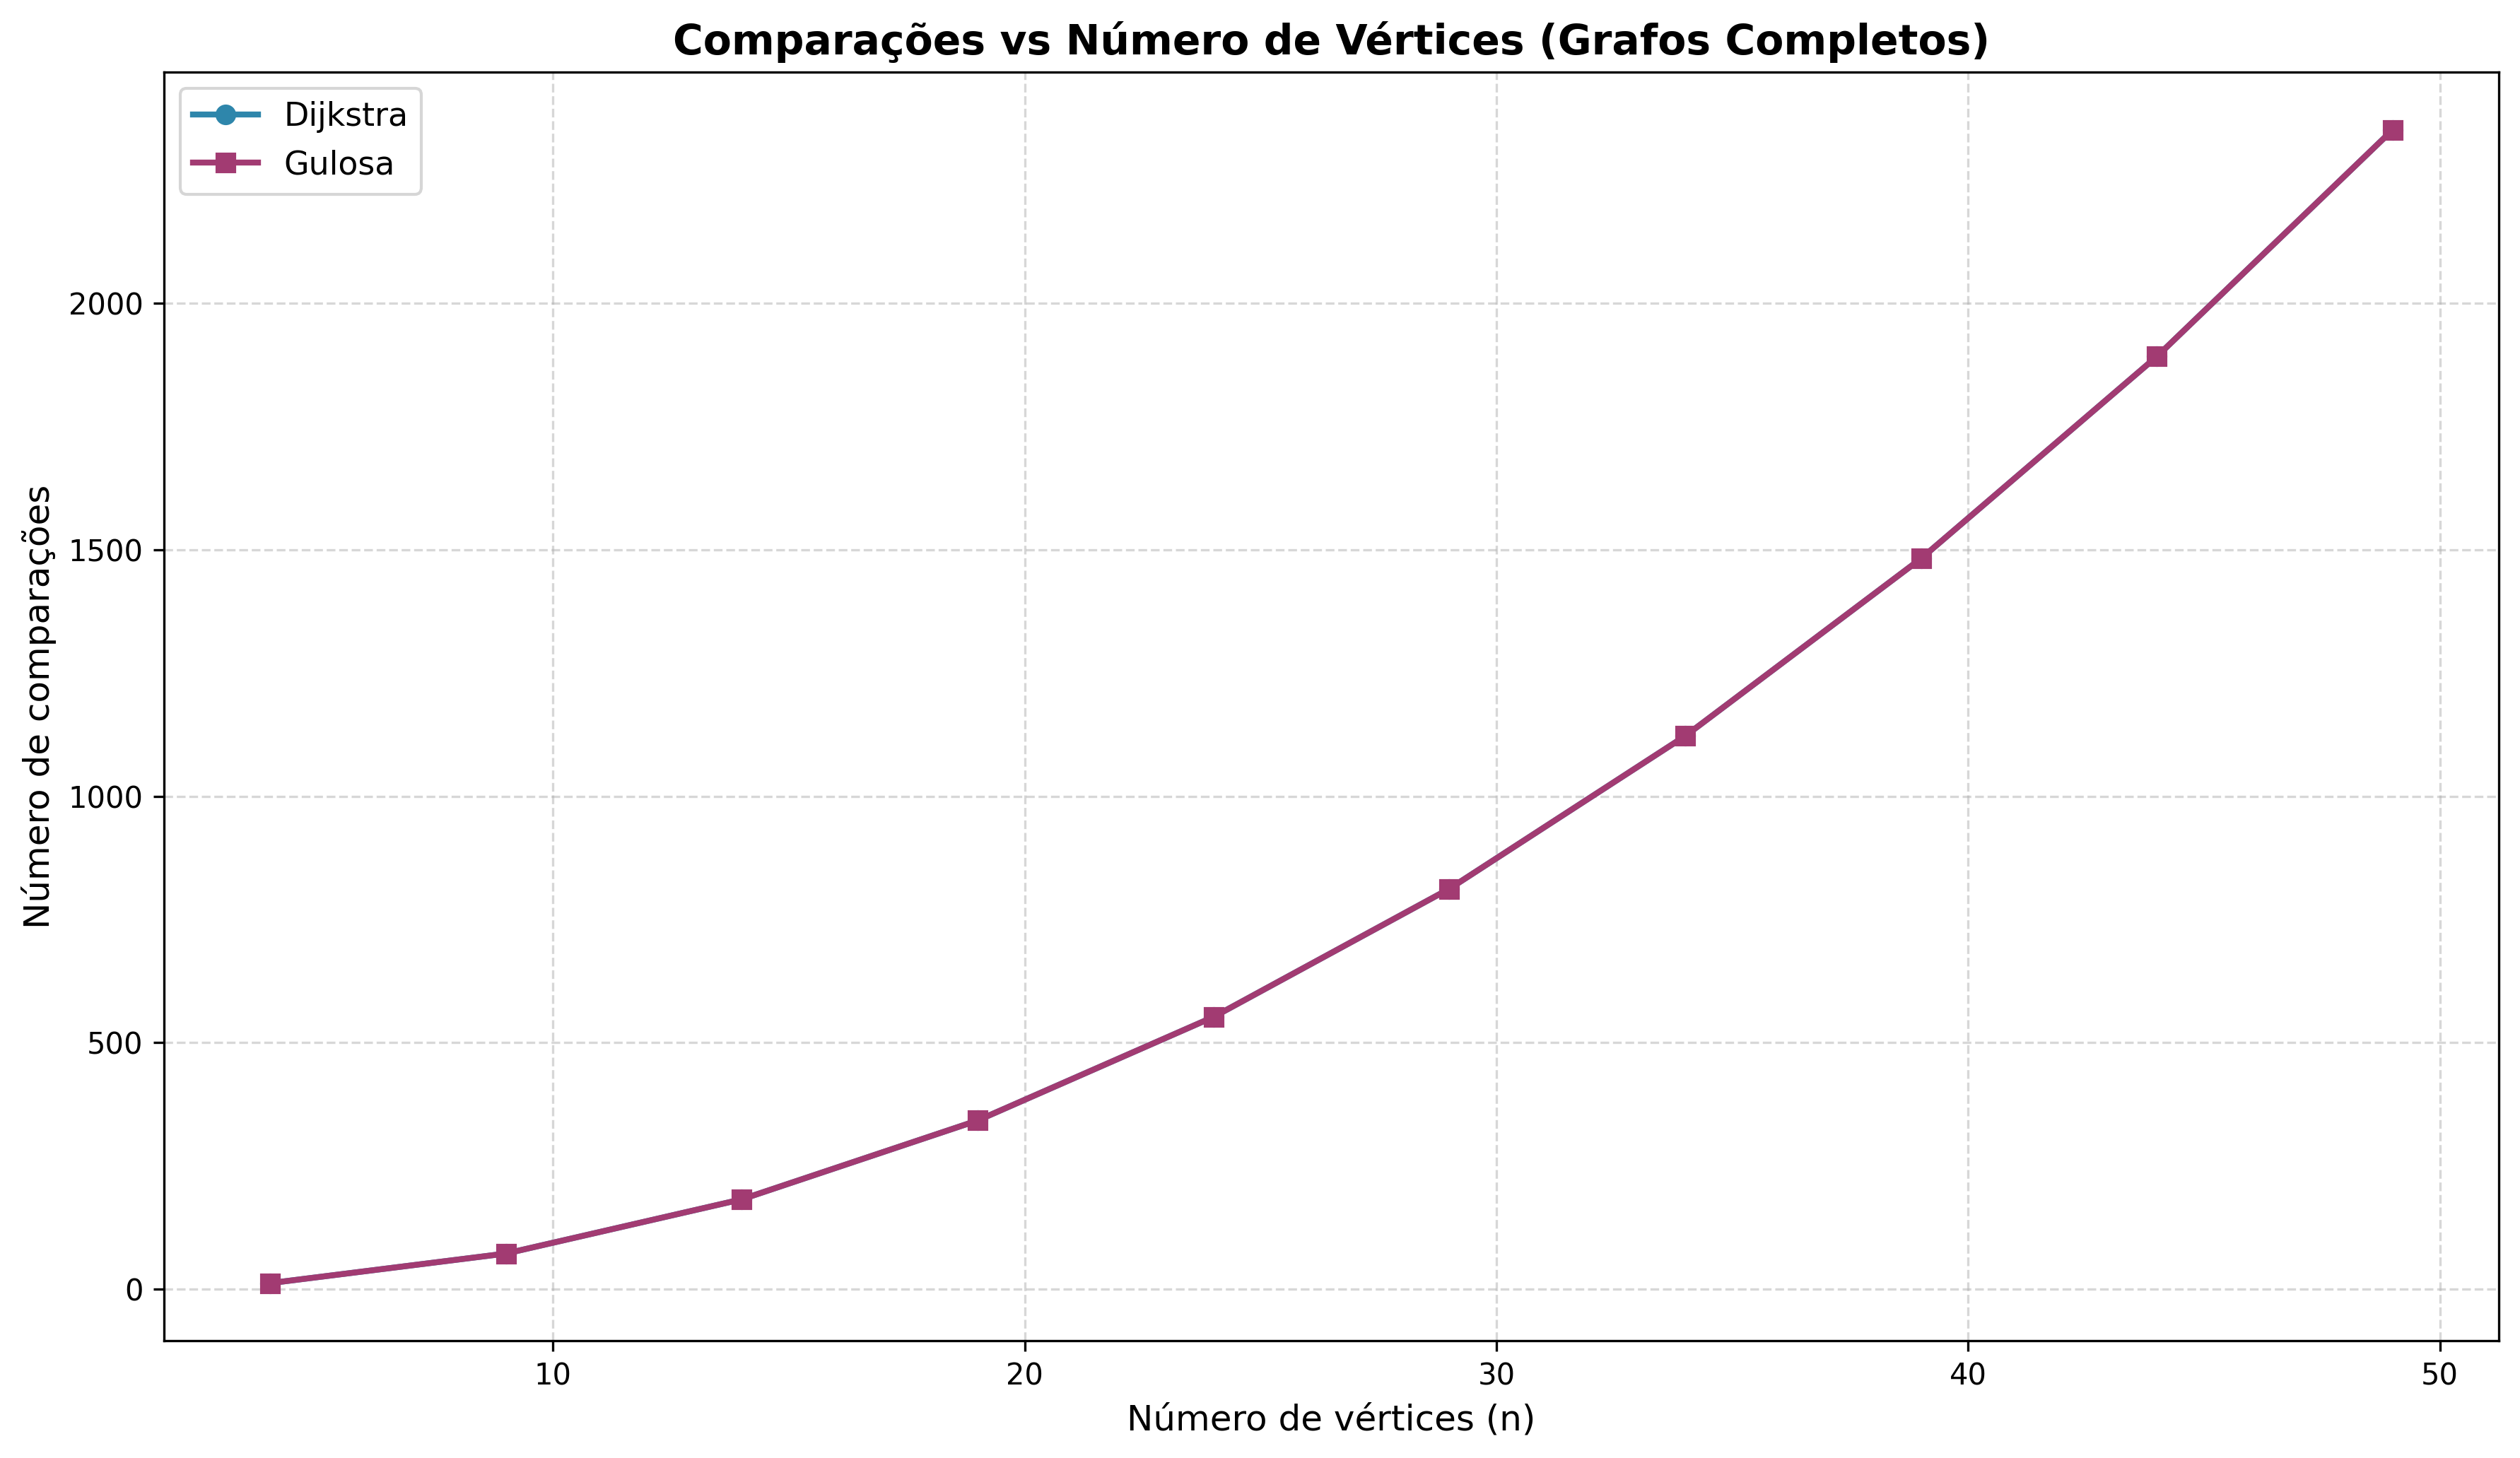
\includegraphics[width=0.85\textwidth]{img/comparacoes_grafos_completos.png}
    \caption{Comparações realizadas por Dijkstra e Gulosa em grafos completos.}
    \label{fig:completos}
\end{figure}

\textbf{Observações}:
\begin{itemize}
    \item O algoritmo de Dijkstra apresenta crescimento aproximadamente quadrático, como esperado para grafos completos ($O(V^2 \log V)$ comparações no pior caso).
    \item A heurística gulosa também apresenta crescimento similar, mas pode realizar mais ou menos comparações dependendo da estrutura do grafo e dos pesos.
\end{itemize}

\subsection{Instâncias do Moodle}

A Tabela~\ref{tab:instancias} apresenta o número de comparações realizadas nas instâncias fornecidas.

\begin{table}[htbp]
    \centering
    \caption{Número de comparações nas instâncias do Moodle.}
    \label{tab:instancias}
    \begin{tabular}{@{}lrr@{}}
        \toprule
        \textbf{Instância} & \textbf{Dijkstra} & \textbf{Gulosa} \\
        \midrule
        10.000 vértices    & [PREENCHER] & [PREENCHER] \\
        1.000.000 vértices & [PREENCHER] & [PREENCHER] \\
        \bottomrule
    \end{tabular}
\end{table}

\textbf{Instruções para preenchimento}: Execute as células correspondentes no notebook e copie os valores impressos para esta tabela.

\section{Análise e Discussão}

\subsection{Complexidade Teórica}

\begin{itemize}
    \item \textbf{Dijkstra}: $O((V + E) \log V)$ com heap binário. Em grafos completos, $E = O(V^2)$, resultando em $O(V^2 \log V)$.
    \item \textbf{Heurística Gulosa}: Também utiliza heap, mas a estratégia de escolha de arestas pode levar a um número diferente de operações. No pior caso, pode explorar todas as arestas, resultando em complexidade similar.
\end{itemize}

\subsection{Resultados Experimentais}

Os experimentos confirmam o crescimento aproximadamente quadrático em grafos completos. A heurística gulosa não garante otimalidade, mas em alguns casos pode realizar um número competitivo de comparações.

\subsection{Corretude}

\begin{itemize}
    \item \textbf{Dijkstra}: garante caminho mínimo correto para pesos não-negativos.
    \item \textbf{Gulosa}: \textbf{não garante} corretude em geral. Foi implementada apenas para fins de comparação experimental.
\end{itemize}

\section{Conclusão}

Este trabalho implementou e comparou o algoritmo de Dijkstra com uma heurística gulosa para o problema de caminho mínimo. Os resultados mostram que:

\begin{enumerate}
    \item Dijkstra apresenta crescimento previsível e ótimo para pesos não-negativos.
    \item A heurística gulosa pode ter desempenho variável dependendo da estrutura do grafo.
    \item A métrica de comparações permite avaliar o esforço computacional de forma independente da implementação.
\end{enumerate}

O código-fonte completo está disponível no notebook Jupyter anexado a este relatório.

\section{Anexos}

\subsection{Código Fonte}

O código completo está disponível em:
\begin{verbatim}
praticas/pratica01/pratica01_experimentos.ipynb
\end{verbatim}

\subsection{Instruções de Execução}

\begin{enumerate}
    \item Ativar ambiente virtual: \texttt{uv sync} (ou equivalente).
    \item Abrir o notebook: \texttt{jupyter notebook pratica01\_experimentos.ipynb}.
    \item Executar as células na ordem.
    \item Os gráficos são salvos automaticamente em \texttt{relatorio/img/}.
\end{enumerate}

\end{document}
